%!TEX root = mainfile.tex

% \section{Determining Redshift} % (fold)
% \label{sub:determingin_redshift}
% 	Section~\ref{sec:contaminants} will describe how contaminants could be eliminated from the large number of potential high redshift galaxies. Taking the remaining objects, the following methods are used to check whether they are in fact LBGs.
	\subsection{Filters and the Dropout Technique} % (fold)
		\label{ssub:filters_and_the_dropout_technique}
		Using photometry, the redshift of a LBG can be estimated using the dropout technique: The flux from the galaxy can be measured in three different bands, ideally two above and one below the Lyman break. If the galaxy is a high redshift Lyman break galaxy, it would be expected that, so long as the filters were correct for the redshift expected, one image would not see the galaxy whereas the other two would observe flux. Below in Figure~\ref{fig:drop_out_at_z7}, the dropout technique is shown for a model galaxy of redshift seven.
		\begin{figure}[!htbp]
			\centering
			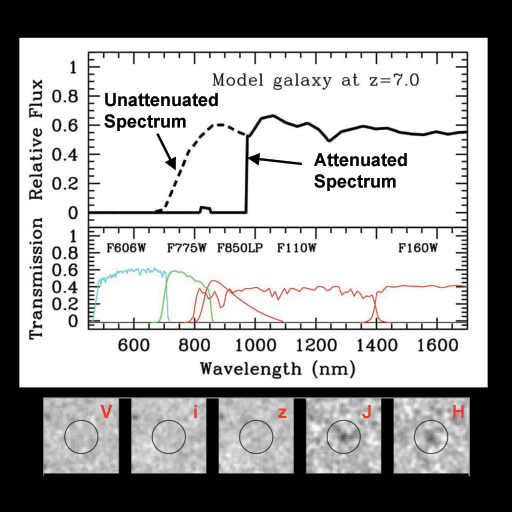
\includegraphics[width=0.5\textwidth]{../Images/drop_out_at_z7.png}
			\caption{Dropout technique for model redshift 7 galaxy\cite{first_galaxies_dropout_at_z7}.\label{fig:drop_out_at_z7}}
		\end{figure}

		The neutral hydrogen has attenuated almost all flux at wavelengths shorter than approximately 1 micrometre. The galaxy has been imaged in several different bands, and the longer wavelength filters show flux, whereas those at wavelengths corresponding to blue-ward of Lyman alpha do not. The galaxies that the group look to study have been shifted such that the drop happens in the infrared. The wavelength of the drop can be worked out using the known rest wavelength of Lyman alpha, as well as the factor by which the wavelength shifts due to the expansion of the universe, as shown in Equation~\ref{eq:dropout_wavelength}.
		\begin{align}
			\text{Rest wavelength of Lyman alpha} \times (1+z) &= \text{observed wavelength of drop}\label{eq:dropout_wavelength}
		\end{align}

		Since the rest wavelength of Lyman alpha is known and the observed wavelength of the drop can be measured, the redshift of the galaxy can be determined. This
		is only a rough estimate when doing photometry since the flux is simply a number in each of the bands. For example, if the bands do not overlap, and the drop happens between two bands, it will not be known at what point the drop occurred, only the range in which it occurred. This motivates the use of bands which are close together or potentially even overlapping. Figure~\ref{fig:filter-systems} shows some different bands and their bandwidth, for different filter systems. Johnson-Cousins- Glass is one of the oldest and still the most commonly used system\cite{BasicObservationalKnowledge}.
		\begin{figure}[!htbp]
			\centering
			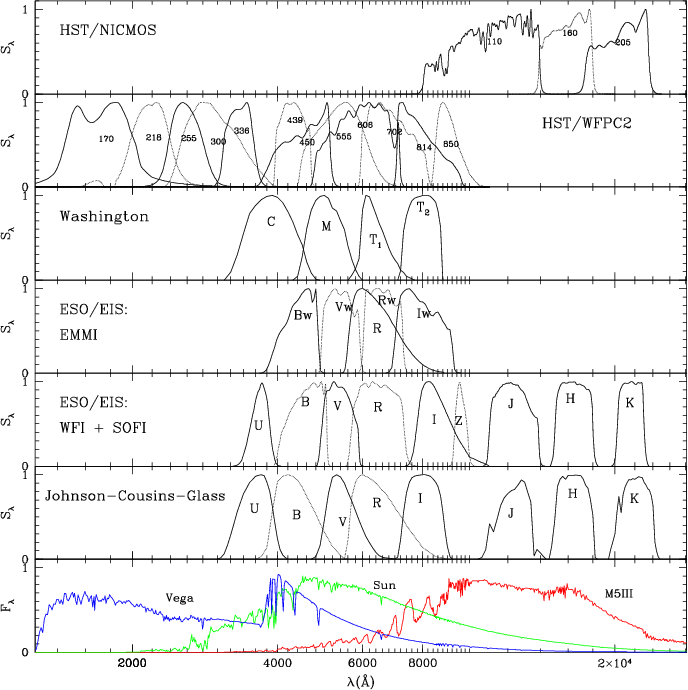
\includegraphics[width=0.65\textwidth]{../Images/filter-systems.png}
			\caption{Various filtering systems\cite{refId0}.\label{fig:filter-systems}}
		\end{figure}

		The bandwidth (or passband) is the wavelength range that can pass through the filter. Filters in different parts of the spectrum are given a common name, for example I band at \SI{806}{\nano\metre}. When observing LBGs, it is beneficial to have three filters in a row so that the position of the drop can be more accurately measured. As can be seen, there are gaps between the J H and K filters, meaning if the drop occurs between J and H, full flux should be observed in H and K and virtually no flux should be seen in J. (the panels beneath Figure~\ref{fig:filter-systems} show an image (or lack thereof) of the $z=7$ galaxy in each of the V, I, z, J and H bands)

		Table~\ref{tab:filter_characteristics} below shows a list of filter names, the central wavelength of that filter, the bandwidth the filter covers, and range of redshifts for which the Lyman alpha drop would be covered. (This  range assumes the bandwidth covers 50\% either side of the central wavelength)
		\begin{table}[!htbp]
			\begin{center}
				\begin{tabular}{c|c|c|c}
					Filter 	& Central wavelength & Bandwidth & Redshift coverage \\
					\hline \hline
					V 	& \SI{551}{\nano\metre}	 & \SI{88}{\nano\metre} & 3.17--3.90 \\
					i 	& \SI{806}{\nano\metre}	 & \SI{149}{\nano\metre} & 5.01--7.25 \\
					Y 	& \SI{1020}{\nano\metre} & \SI{120}{\nano\metre} & 6.90--7.88 \\
					J 	& \SI{1220}{\nano\metre} & \SI{213}{\nano\metre} & 9.16--9.91 \\
					H 	& \SI{1630}{\nano\metre} & \SI{307}{\nano\metre} & 11.14--13.67 \\
					K 	& \SI{2190}{\nano\metre} & \SI{390}{\nano\metre} & 15.41--18.61
				\end{tabular}
			\end{center}
			\caption{Data highlighting which filters would be useful for observing particular redshift galaxies\cite{Galactic_Astronomy_Binney_Merrifield}}
			\label{tab:filter_characteristics}
		\end{table}

		Table~\ref{tab:filter_characteristics} must be taken into consideration that two filters should be red-ward of the drop and one blue-ward. One the fluxes have been measured in all three bands, if the object is indeed a LBG, there should be a sharp drop in flux in  one of the bands. However this does not totally rule out other possibilities: Some other objects could also exhibit a drop in flux, posing as LBGs, so usually a follow up method is used, and this is spectroscopy. Spectroscopy The drop out technique provides a good indication that a galaxy is a high redshift Lyman break galaxy, however the best way to confirm this is with spectroscopy.
		% subsection filters_and_the_dropout_technique (end)

% subsection determining_redshift (end)
